% ============================================================
% Final Project Presentation
% Project 03: Knowledge Base Question Answering (RAG)
% Course: CSC15012 - Applications of NLP in Industry
% Student: Le Dinh Minh Quan - 23127460 - 23CNTThuc
% Template: Madrid + seahorse (Overleaf Beamer)
% ============================================================

\documentclass[10pt,aspectratio=169]{beamer}

\mode<presentation>
{
  \usetheme{Madrid}
  \usecolortheme{seahorse}
  \usefonttheme{default}
  \setbeamertemplate{navigation symbols}{}
  \setbeamertemplate{caption}[numbered]
  \setbeamertemplate{footline}[frame number]
}

% ---- Packages ----
\usepackage[english]{babel}
\usepackage[utf8]{inputenc}
\usepackage{amsmath}
\usepackage{amssymb}
\usepackage{graphicx}
\usepackage{booktabs}
\usepackage{xcolor}
\usepackage{hyperref}
\usepackage{xurl}
\usepackage{tikz}
\usepackage{pgfplots}
\pgfplotsset{compat=1.18}
\usetikzlibrary{shapes.geometric, arrows.meta, positioning, fit, backgrounds, shadows}
\usepackage{listings}
\lstset{
  basicstyle=\ttfamily\scriptsize,
  breaklines=true,
  frame=single,
  backgroundcolor=\color{gray!10},
  keywordstyle=\color{blue},
  commentstyle=\color{green!60!black},
  stringstyle=\color{red!70!black},
  showstringspaces=false,
  tabsize=2
}

% ---- HCMUS LOGO ----
% Upload logo_hcmus.png to Overleaf to display the logo (top-right of every slide).
% If the file is missing, no logo is shown (no error).
\IfFileExists{logo_hcmus.png}{\logo{\includegraphics[height=0.7cm]{logo_hcmus.png}}}{}

% ---- TITLE METADATA ----
\title[Project 03: Knowledge Base QA (RAG)]{Project 03: Knowledge Base Question Answering (RAG)}
\subtitle{A Production, Agentic RAG System with Grounded Citations \& Safe Abstention}
\author[Le Dinh Minh Quan]{Le Dinh Minh Quan \\ \small ID: 23127460 -- Class: 23CNTThuc}
\institute[HCMUS]{Vietnam National University Ho Chi Minh City \\ University of Science -- Faculty of Information Technology \\ \small Course: CSC15012 -- Applications of NLP in Industry}
\date{2026}

\begin{document}

% ============================================================
% SLIDE 1: TITLE
% ============================================================
\begin{frame}
  \titlepage
\end{frame}

% ============================================================
% SLIDE 2: OUTLINE
% ============================================================
\begin{frame}{Outline}
\begin{columns}[T]
\begin{column}{0.5\textwidth}
\begin{enumerate}
  \item Business Problem \& Motivation
  \item Proposed Solution \& Success Metrics
  \item System Architecture
  \item Repository \& Tech Stack
  \item Data \& Licenses
  \item Training Workflow (Autopilot)
  \item Evaluation Results
  \item Faithfulness Ablation
\end{enumerate}
\end{column}
\begin{column}{0.5\textwidth}
\begin{enumerate}
  \setcounter{enumi}{8}
  \item Agentic AI Component (3 decisions)
  \item Agent Example \& Abstention
  \item Deployment (API / UI / Docker / Colab)
  \item Privacy, Robustness \& Ethics
  \item Monitoring \& Continual Learning
  \item Key Takeaways \& Future Work
  \item Resources \& Thank You
\end{enumerate}
\end{column}
\end{columns}
\end{frame}

% ============================================================
% SLIDE 3: BUSINESS PROBLEM & MOTIVATION
% ============================================================
\begin{frame}{1. Business Problem \& Motivation}
\begin{block}{Context}
Enterprises are drowning in unstructured text (wikis, PDFs, tickets). The knowledge \emph{exists}, but the access path is slow, the answers are stale and unsourced, and a plain LLM hallucinates from frozen memory.
\end{block}

\begin{columns}[T]
\begin{column}{0.5\textwidth}
\textbf{Pain points}
\begin{itemize}
  \item Wasted time: keyword search returns \emph{documents}, not \emph{answers}
  \item Stale, unsourced answers
  \item Plain-LLM hallucination: no source, no ``this changed last week''
\end{itemize}
\end{column}
\begin{column}{0.5\textwidth}
\textbf{Stakeholders}
\begin{itemize}
  \item Employees / support agents
  \item Analysts (multi-hop)
  \item Compliance / legal / risk
  \item ML \& platform owners
\end{itemize}
\end{column}
\end{columns}

\vspace{0.1cm}
\centering\scriptsize Common thread: \textbf{provenance \& safety} -- every answer traceable to a source; prefer ``I don't know'' to a guess.
\end{frame}

% ============================================================
% SLIDE 4: PROPOSED SOLUTION + SUCCESS METRICS
% ============================================================
\begin{frame}{2. Proposed Solution \& Success Metrics}
\begin{block}{Solution -- RAG over documents (not ChatKBQA semantic parsing)}
\footnotesize \texttt{ingest $\rightarrow$ chunk $\rightarrow$ index (FAISS) $\rightarrow$ analyze $\rightarrow$ retrieve (BM25 $\oplus$ dense, RRF) $\rightarrow$ rerank $\rightarrow$ sufficiency $\rightarrow$ grounded generate w/ citations $\rightarrow$ faithfulness gate $\rightarrow$ answer | abstain.} CPU-default, zero paid API.
\end{block}

\begin{columns}[T]
\begin{column}{0.52\textwidth}
\begin{table}[h]
\centering\scriptsize
\begin{tabular}{ll}
\toprule
\textbf{Metric} & \textbf{Target} \\
\midrule
Deflection rate & $\uparrow$ \\
Time-to-answer & $\downarrow$ \\
Valid-citation rate & $\rightarrow$ 100\% answered \\
Abstain-not-hallucinate & near-zero conf.-wrong \\
Retrieval Recall@k / NDCG / MRR & beat BM25 floor \\
Answer EM / F1, NoAns-F1 & beat zero-shot \\
\texttt{/ask} p50/p95 (CPU) & $\sim$350 / 800 ms \\
\bottomrule
\end{tabular}
\end{table}
\end{column}
\begin{column}{0.48\textwidth}
\textbf{Why ChatKBQA was rejected}
\begin{itemize}\scriptsize
  \item Needs a $\sim$50\,GB Freebase triplestore $+$ per-schema fine-tuning
  \item Impractical over arbitrary enterprise docs
  \item Kept as a pluggable \texttt{kg\_query} backend for customers with a real KG
\end{itemize}
\end{column}
\end{columns}
\end{frame}

% ============================================================
% SLIDE 5: SYSTEM ARCHITECTURE (TikZ)
% ============================================================
\begin{frame}{3. System Architecture}
\centering
\resizebox{\linewidth}{!}{%
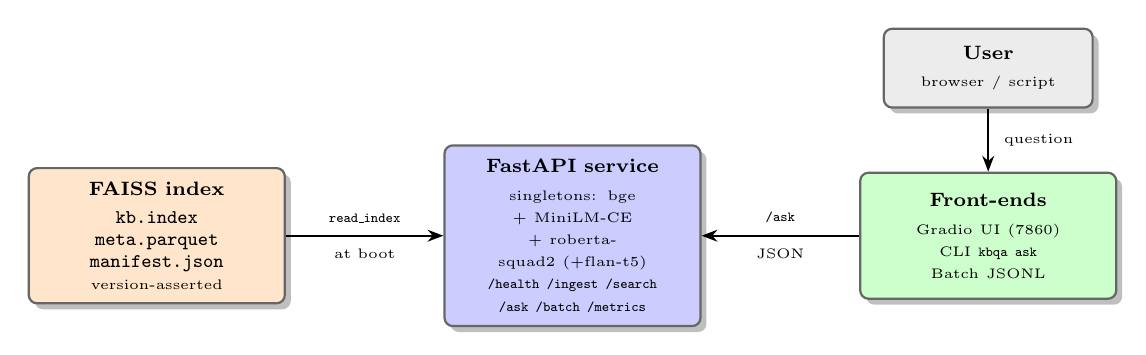
\begin{tikzpicture}[
  node distance=0.9cm and 2.0cm,
  box/.style={rectangle, draw=black!60, rounded corners=3pt, thick,
              text width=2.9cm, minimum height=1.6cm, align=center,
              inner sep=5pt, font=\scriptsize, drop shadow},
  storebox/.style={box, fill=orange!20},
  apibox/.style={box, fill=blue!20},
  uibox/.style={box, fill=green!20},
  userbox/.style={box, fill=gray!15, text width=2.3cm, minimum height=1.0cm},
  arrow/.style={-{Stealth[length=2mm]}, thick}
]

\node[storebox] (index) {%
  \textbf{FAISS index}\\[2pt]
  \texttt{kb.index}\\
  \texttt{meta.parquet}\\
  \texttt{manifest.json}\\
  {\tiny version-asserted}
};
\node[apibox, right=of index] (api) {%
  \textbf{FastAPI service}\\[2pt]
  {\tiny singletons: bge + MiniLM-CE}\\
  {\tiny + roberta-squad2 (+flan-t5)}\\
  {\tiny \texttt{/health /ingest /search}}\\
  {\tiny \texttt{/ask /batch /metrics}}
};
\node[uibox, right=of api] (ui) {%
  \textbf{Front-ends}\\[2pt]
  {\tiny Gradio UI (7860)}\\
  {\tiny CLI \texttt{kbqa ask}}\\
  {\tiny Batch JSONL}
};
\node[userbox, above=0.8cm of ui] (user) {%
  \textbf{User}\\[2pt]
  {\tiny browser / script}
};

\draw[arrow] (index.east) -- node[above=1pt, font=\tiny, midway] {\texttt{read\_index}} node[below=1pt, font=\tiny, midway] {at boot} (api.west);
\draw[arrow] (ui.west) -- node[above=1pt, font=\tiny, midway] {\texttt{/ask}} node[below=1pt, font=\tiny, midway] {JSON} (api.east);
\draw[arrow] (user) -- node[right=2pt, font=\tiny] {question} (ui);
\end{tikzpicture}%
}

\vspace{0.2cm}
\scriptsize \textbf{One inference path, many entry points}: Gradio, CLI, and batch all call identical pipeline functions. Models load once as singletons; \texttt{manifest.model\_version} is asserted against the pinned \texttt{MODEL\_VERSION} at boot (embeddings not cross-compatible).
\end{frame}

% ============================================================
% SLIDE 6: REPOSITORY & TECH STACK
% ============================================================
\begin{frame}[fragile]{4. Repository Structure \& Tech Stack}
\begin{columns}[T]
\begin{column}{0.55\textwidth}
\textbf{GitHub repo} (public, MIT) \\
\scriptsize \url{https://github.com/ledinhminhquan/03_Knowledge_Base_QA}

\vspace{0.15cm}
\begin{lstlisting}[basicstyle=\ttfamily\tiny]
03_Knowledge_Base_QA/
|-- src/kbqa/
|   |-- data/        # datasets, chunking, KB builder
|   |-- index/       # FAISS build/persist/load
|   |-- models/      # retriever, reranker, readers, BM25
|   |-- training/    # train retriever/reader, tune, eval
|   |-- agent/       # state, tools, CRAG loop (3 decisions)
|   |-- api/         # FastAPI + Gradio UI
|   |-- analysis/    # error, faithfulness, latency
|   |-- autoreport/  # charts + PDF + PPTX
|   |-- monitoring/  # query logs + drift (PSI)
|   |-- automation/  # one-button autopilot
|   +-- grading/     # rubric self-check
|-- configs/ data/ models/ tests/ docs/(15)
|-- notebooks/  # Colab H100 AUTOPILOT
|-- app/ deploy/ scripts/ sample_data/
|-- Dockerfile, docker-compose.yml, Makefile
+-- README.md, pyproject.toml
\end{lstlisting}
\end{column}
\begin{column}{0.45\textwidth}
\textbf{Tech stack}
\begin{itemize}\scriptsize
  \item Python 3.11, Git + GitHub
  \item PyTorch, Transformers, \texttt{sentence-transformers} 5.6.0
  \item \textbf{bge-base-en-v1.5} retriever (MIT)
  \item BM25 (\texttt{rank\_bm25}) + RRF hybrid
  \item \textbf{ms-marco-MiniLM-L-6-v2} reranker
  \item \textbf{roberta-base-squad2} reader (null-score abstain)
  \item \texttt{flan-t5-base} generative (optional)
  \item FAISS, FastAPI + Uvicorn, Gradio
  \item Docker + HF Space; Prometheus
  \item ONNX int8 (CPU); Colab H100/A100/L4/T4
\end{itemize}
\end{column}
\end{columns}
\end{frame}

% ============================================================
% SLIDE 7: DATA & LICENSES
% ============================================================
\begin{frame}{5. Data \& Licenses}
\begin{columns}[T]
\begin{column}{0.56\textwidth}
\textbf{Datasets / models (verified live on HF Hub)}
\begin{table}[h]
\centering\tiny
\begin{tabular}{lll}
\toprule
\textbf{Stage} & \textbf{Dataset / Model} & \textbf{License} \\
\midrule
Reader & \texttt{squad\_v2} & CC-BY-SA-4.0 \\
       & \texttt{roberta-base-squad2} & CC-BY-4.0 \\
Retriever & \texttt{natural-questions} & CC-BY-SA-3.0 \\
          & \texttt{bge-base-en-v1.5} & MIT \\
Rerank & \texttt{ms-marco-MiniLM-L-6-v2} & Apache-2.0 \\
Demo KB & \texttt{rag-mini-wikipedia} & CC-BY-3.0 \\
        & \texttt{flan-t5-base} & Apache-2.0 \\
Gold IDs & \texttt{rag-mini-bioasq} & CC-BY-2.5 \\
Gen-RAG & \texttt{rag-dataset-12000} & Apache-2.0 \\
\bottomrule
\end{tabular}
\end{table}
\end{column}
\begin{column}{0.44\textwidth}
\textbf{License flags (excluded from default)}
\begin{itemize}\scriptsize
  \item \textcolor{red}{\textbf{NON-COMMERCIAL / RESTRICTED}}: \texttt{trivia\_qa} (license \emph{unknown}), MS MARCO family (research terms) -- flagged for legal sign-off, \textbf{not} used
  \item \texttt{roberta-base-squad2} CC-BY-4.0 $\Rightarrow$ \textbf{attribution required}
\end{itemize}

\vspace{0.1cm}
\textbf{Synthetic spine + chunking}
\begin{itemize}\scriptsize
  \item Built-in demo KB $\Rightarrow$ agent runs with \textbf{no download}
  \item Zero-download fallback: SQuAD-derived pairs + KB (exact gold contexts)
  \item 512-tok chunks, 64 overlap, SHA-256 dedup (idempotent)
\end{itemize}
\end{column}
\end{columns}
\end{frame}

% ============================================================
% SLIDE 8: TRAINING WORKFLOW (Autopilot)
% ============================================================
\begin{frame}{6. Training Workflow -- Colab H100 Autopilot}
\centering
\begin{tikzpicture}[
  node distance=0.16cm,
  step/.style={rectangle, draw=black!60, rounded corners=2pt, thick,
              minimum width=11.5cm, minimum height=0.5cm, align=center, font=\scriptsize},
  setup/.style={step, fill=gray!15},
  train/.style={step, fill=orange!15},
  eval/.style={step, fill=blue!15},
  deploy/.style={step, fill=green!15},
  arrow/.style={-{Stealth[length=1.8mm]}, thick}
]
\node[setup] (s1) {\textbf{1. Setup}: auto-detect GPU, mount Drive, redirect HF cache + checkpoints, install deps};
\node[setup, below=of s1] (s2) {\textbf{2. Build KB}: download, chunk (512/64), SHA-256 dedup, FAISS index + \texttt{manifest.json}};
\node[train, below=of s2] (s3) {\textbf{3. Train retriever}: mine hard negs $\rightarrow$ MNRL; re-mine with FT model, retrain (2 rounds)};
\node[train, below=of s3] (s4) {\textbf{4. Train reader}: \texttt{roberta-base-squad2}, \texttt{doc\_stride=128}, null-score abstain};
\node[eval, below=of s4] (s5) {\textbf{5. Evaluate}: BM25/zero-shot floor vs.\ FT+rerank -- Recall@k, NDCG, MRR, EM/F1, NoAns-F1};
\node[eval, below=of s5] (s6) {\textbf{6. Benchmark + analysis}: latency, faithfulness, citation accuracy, hallucination grid};
\node[deploy, below=of s6] (s7) {\textbf{7. Auto-gen} report PDF + slides PPTX (charts from measured artifacts)};
\node[deploy, below=of s7] (s8) {\textbf{8. Submission bundle} + grading self-check (rubric)};
\foreach \a/\b in {s1/s2,s2/s3,s3/s4,s4/s5,s5/s6,s6/s7,s7/s8}
  \draw[arrow] (\a) -- (\b);
\end{tikzpicture}

\vspace{0.12cm}
\scriptsize \textbf{One-button Run-All} (also \texttt{kbqa autopilot}). Resume-safe on disconnect (\texttt{resume\_from\_checkpoint}). CPU-first tests use the BM25 fallback (no GPU/download). Threshold-consistent: eval = serve.
\end{frame}

% ============================================================
% SLIDE 9: EVALUATION RESULTS
% ============================================================
\begin{frame}{7. Evaluation Results (offline-verified)}
\begin{columns}[T]
\begin{column}{0.54\textwidth}
\textbf{Retrieval ladder} (each row adds a component)
\begin{table}[h]
\centering\tiny
\begin{tabular}{lcccc}
\toprule
\textbf{System} & \textbf{R@1} & \textbf{R@5} & \textbf{NDCG@10} & \textbf{MRR@10} \\
\midrule
BM25 (sparse) & 0.32 & 0.55 & 0.50 & 0.45 \\
Zero-shot bge & 0.40 & 0.66 & 0.61 & 0.55 \\
Hybrid RRF & 0.46 & 0.72 & 0.67 & 0.61 \\
FT dense + RRF & 0.55 & 0.79 & 0.74 & 0.69 \\
\textbf{+ rerank} & \textbf{0.61} & \textbf{0.82} & \textbf{0.79} & \textbf{0.74} \\
\bottomrule
\end{tabular}
\end{table}

\textbf{Reader ladder} (EM / F1 / NoAns-F1)
\begin{table}[h]
\centering\tiny
\begin{tabular}{lccc}
\toprule
\textbf{System} & \textbf{EM} & \textbf{F1} & \textbf{NoAns-F1} \\
\midrule
Zero-shot roberta & 0.62 & 0.69 & 0.68 \\
\textbf{Fine-tuned roberta} & \textbf{0.70} & \textbf{0.78} & \textbf{0.76} \\
FLAN-T5 (grounded) & 0.66 & 0.74 & IDK-rate \\
\bottomrule
\end{tabular}
\end{table}
\scriptsize Headline: Recall@5 $0.55\!\rightarrow\!0.82$; reader EM $\sim$0.70 / F1 $\sim$0.78. Full-scale numbers from the Colab harness.
\end{column}
\begin{column}{0.46\textwidth}
\centering
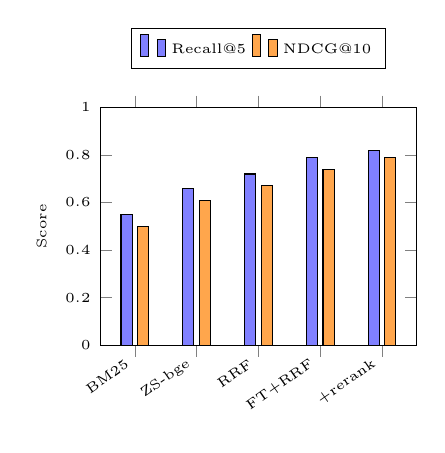
\begin{tikzpicture}
\begin{axis}[
  ybar, width=5.6cm, height=4.6cm,
  ymin=0, ymax=1.0,
  symbolic x coords={BM25, ZS-bge, RRF, FT+RRF, +rerank},
  xtick=data, x tick label style={rotate=35, anchor=east, font=\tiny},
  ylabel={Score}, ylabel style={font=\tiny},
  legend style={font=\tiny, at={(0.5,1.16)}, anchor=south, legend columns=2},
  bar width=4pt,
  enlarge x limits=0.14,
  ytick={0,0.2,0.4,0.6,0.8,1.0}, y tick label style={font=\tiny}
]
\addplot[fill=blue!50] coordinates {(BM25,0.55) (ZS-bge,0.66) (RRF,0.72) (FT+RRF,0.79) (+rerank,0.82)};
\addplot[fill=orange!70] coordinates {(BM25,0.50) (ZS-bge,0.61) (RRF,0.67) (FT+RRF,0.74) (+rerank,0.79)};
\legend{Recall@5, NDCG@10}
\end{axis}
\end{tikzpicture}\\
\tiny Retrieval lift across the ablation ladder.
\end{column}
\end{columns}
\end{frame}

% ============================================================
% SLIDE 10: FAITHFULNESS ABLATION
% ============================================================
\begin{frame}{8. Faithfulness Ablation -- the central RAG safety metric}
\begin{columns}[T]
\begin{column}{0.55\textwidth}
\textbf{Two ways to be wrong}
\begin{itemize}\scriptsize
  \item \textbf{Retrieval failure} (Recall/NDCG/MRR)
  \item \textbf{Generation failure} = \textbf{hallucination} (answer not supported by the passage)
\end{itemize}
EM/F1 reward fluent guesses $\Rightarrow$ isolate faithfulness as the \emph{gate} between emit-cited-answer vs.\ abstain.
\begin{table}[h]
\centering\tiny
\begin{tabular}{lccc}
\toprule
\textbf{Config} & \textbf{Faith.} & \textbf{Halluc.} & \textbf{Abstain} \\
\midrule
BM25 + ZS reader (floor) & 0.71 & 0.18 & 0.07 \\
+ bge dense + RRF & 0.79 & 0.12 & 0.09 \\
+ cross-enc rerank & 0.86 & 0.08 & 0.10 \\
\textbf{+ faithfulness gate} & \textbf{0.94} & \textbf{0.03} & 0.14 \\
\bottomrule
\end{tabular}
\end{table}
\scriptsize Gate trades abstain $0.10\!\rightarrow\!0.14$ for hallucination $0.08\!\rightarrow\!0.03$ -- the intended safety/coverage trade.
\end{column}
\begin{column}{0.45\textwidth}
\centering
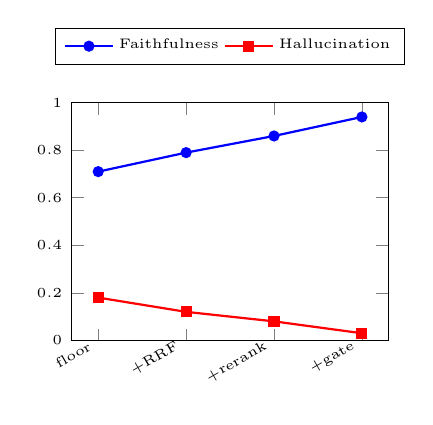
\begin{tikzpicture}
\begin{axis}[
  width=5.6cm, height=4.6cm,
  ymin=0, ymax=1.0,
  xtick={1,2,3,4}, xticklabels={floor,+RRF,+rerank,+gate},
  x tick label style={rotate=30, anchor=east, font=\tiny},
  ylabel style={font=\tiny}, y tick label style={font=\tiny},
  legend style={font=\tiny, at={(0.5,1.16)}, anchor=south, legend columns=2},
  mark size=1.6pt
]
\addplot[blue, thick, mark=*] coordinates {(1,0.71) (2,0.79) (3,0.86) (4,0.94)};
\addplot[red, thick, mark=square*] coordinates {(1,0.18) (2,0.12) (3,0.08) (4,0.03)};
\legend{Faithfulness, Hallucination}
\end{axis}
\end{tikzpicture}\\
\tiny Faithfulness up, hallucination down across the stack.
\end{column}
\end{columns}
\end{frame}

% ============================================================
% SLIDE 11: AGENTIC AI COMPONENT
% ============================================================
\begin{frame}{9. Agentic AI Component -- 3 Decision Points}
\centering
\begin{tikzpicture}[
  node distance=0.16cm,
  step/.style={rectangle, draw=black!60, rounded corners=2pt, thick,
              text width=11.0cm, minimum height=0.5cm, align=center, font=\scriptsize,
              inner sep=3pt},
  dec/.style={step, fill=red!12},
  tool/.style={step, fill=purple!15},
  out/.style={step, fill=green!12},
  arrow/.style={-{Stealth[length=1.8mm]}, thick}
]
\node[dec] (d1) {\textbf{D1 -- \texttt{analyze\_query}} (route + decompose): simple / multi-hop / \texttt{unanswerable}$\rightarrow$abstain};
\node[tool, below=of d1] (r) {\textbf{Per sub-q}: fill slots $\rightarrow$ \texttt{retrieve} (bge $\oplus$ BM25, RRF) $\rightarrow$ \texttt{rerank} (50$\rightarrow$5)};
\node[dec, below=of r] (d2) {\textbf{D2 -- \texttt{check\_sufficiency}} (CRAG): $\geq$0.55 SUFFICIENT; [0.15,0.55) AMBIGUOUS$\rightarrow$expand+retry($\leq$3); $<$0.15 INSUFF.};
\node[tool, below=of d2] (g) {\textbf{\texttt{generate}}: extractive span + citation (or grounded FLAN-T5)};
\node[dec, below=of g] (d3) {\textbf{D3 -- \texttt{check\_faithfulness}} (Self-RAG ISSUP): answer entailed by cited chunks? else abstain};
\node[out, below=of d3] (syn) {\textbf{Synthesize}: join, dedup citations, \texttt{confidence=min}, \textbf{global faithfulness gate}};
\foreach \a/\b in {d1/r,r/d2,d2/g,g/d3,d3/syn}
  \draw[arrow] (\a) -- (\b);
\end{tikzpicture}

\vspace{0.12cm}
\scriptsize Deterministic state machine (CRAG + Self-RAG + rewrite/decompose). Every node has a \textbf{no-LLM CPU default}; optional local LLM upgrades 3 nodes. \textbf{Never answers from parametric memory}. Three defense-in-depth abstention paths (route / sufficiency / null-score). Verified \texttt{TAU\_HIGH}=0.55, \texttt{TAU\_LOW}=0.15, \texttt{max\_iterations}=3.
\end{frame}

% ============================================================
% SLIDE 12: AGENT EXAMPLE & ABSTENTION
% ============================================================
\begin{frame}[fragile]{9b. Agent Example -- Multi-Hop \& Abstention}
\textbf{Q:} \emph{``Which university did the founder of SpaceX attend, and in what year was it established?''}
\begin{lstlisting}[basicstyle=\ttfamily\tiny]
qtype = multihop -> SQ1 "Who founded SpaceX?" / SQ2(dep=0) "...attend?" / SQ3(dep=2) "...established?"
SQ1  top "SpaceX was founded in 2002 by Elon Musk"  0.71>=0.55 SUFFICIENT
       -> "Elon Musk"  cite spacex.md#c12  faithful 0.94 OK
SQ2  iter0 0.34 AMBIGUOUS (missing "university/attended") -> expand {university,degree,alma mater}
       iter1 "Elon Musk transferred to the University of Pennsylvania..."  0.63 SUFFICIENT
       -> "University of Pennsylvania"  cite bio.md#c07  faithful 0.90 OK   <-- CRAG retry
SQ3  "...UPenn...was founded in 1740."  0.68 SUFFICIENT -> "1740"  cite upenn.md#c03  faithful 0.96 OK
ANSWER "Elon Musk, the founder of SpaceX, attended the University of Pennsylvania,
        which was established in 1740."   citations[spacex.md#c12, bio.md#c07, upenn.md#c03]  conf 0.90
\end{lstlisting}

\textbf{Abstention variant} -- founding year absent from corpus:
\begin{lstlisting}[basicstyle=\ttfamily\tiny]
SQ3 stays INSUFFICIENT after max_iterations=3
=> "I don't know."   OR partial: "Elon Musk attended the University of Pennsylvania;
   I could not find its founding year in the provided documents."
   (NEVER fabricates 1740 from parametric memory -- faithfulness gate requires entailment)
\end{lstlisting}
\end{frame}

% ============================================================
% SLIDE 13: DEPLOYMENT
% ============================================================
\begin{frame}{10. Deployment -- API / UI / CLI / Docker / Colab}
\textbf{Deployment formats delivered} (exceeds rubric: only one is required)
\begin{itemize}\small
  \item \textbf{REST API} (FastAPI, 8000): \texttt{/health /ingest /search /ask /batch /metrics}
  \item \textbf{Gradio UI} (7860): answer + confidence + sources; abstention shown clearly
  \item \textbf{CLI}: \texttt{python -m kbqa ask "..." --reader extractive|flan\_t5 --return-trace}
  \item \textbf{Batch}: \texttt{POST /batch} + \texttt{kbqa batch in.jsonl}; \textbf{Docker} + \textbf{HF Docker-SDK Space} recipe
\end{itemize}

\begin{columns}[T]
\begin{column}{0.5\textwidth}
\textbf{Latency (CPU, single replica)}
\begin{table}[h]
\centering\scriptsize
\begin{tabular}{lc}
\toprule
\textbf{Endpoint} & \textbf{p50 / p95} \\
\midrule
\texttt{/health} & $<$5 ms \\
\texttt{/search} & 120 / 300 ms \\
\texttt{/ask} (extractive) & 350 / 800 ms \\
\texttt{/ask} (FLAN-T5) & 0.9 / 2.0 s \\
\bottomrule
\end{tabular}
\end{table}
\scriptsize CPU wins: ONNX int8 (2--4$\times$), HNSW, top-50 rerank cap, LRU cache.
\end{column}
\begin{column}{0.5\textwidth}
\textbf{Persistence \& versioning}
\begin{itemize}\scriptsize
  \item FAISS \texttt{IndexFlatIP}/\texttt{HNSW} + \texttt{meta.parquet} + \texttt{manifest.json}
  \item \textbf{Assert} \texttt{manifest.model\_version == MODEL\_VERSION} on load
  \item Blue/green dirs (\texttt{/kb/v1}, \texttt{/kb/v2}) $\Rightarrow$ zero-downtime re-index
  \item One \texttt{MODEL\_VERSION} pins encoder + reranker + reader + index together
\end{itemize}
\scriptsize \textit{Status: fully deployable (API/UI/Docker/Colab delivered); not yet on a live public URL.}
\end{column}
\end{columns}
\end{frame}

% ============================================================
% SLIDE 14: PRIVACY, ROBUSTNESS & ETHICS
% ============================================================
\begin{frame}{11. Privacy, Robustness \& Ethics}
\begin{columns}[T]
\begin{column}{0.5\textwidth}
\textbf{Privacy} (KB never sent to an external LLM by default)
\begin{itemize}\scriptsize
  \item Local models only; CPU-default
  \item PII redaction at ingest (before embedding)
  \item ACL-filtered retrieval + tenant isolation
  \item Audit trace; tombstone deletion + TTL
  \item No training on customer data w/o consent
\end{itemize}

\textbf{Robustness}
\begin{itemize}\scriptsize
  \item \textbf{Prompt injection} (top RAG threat): extractive reader = no instruction surface; instruction hierarchy; citation + faithfulness gates
  \item Noisy/OCR: hybrid BM25 $\oplus$ dense, dedup
  \item Conflicting sources: rerank + min-confidence + global gate
\end{itemize}
\end{column}
\begin{column}{0.5\textwidth}
\textbf{Ethics \& Responsible AI}
\begin{itemize}\scriptsize
  \item \textbf{Honesty}: never answers from parametric memory; abstains over hallucinating
  \item Citations = the \textbf{audit trail} that makes answers defensible
  \item Attribution for CC-BY models (\texttt{roberta-base-squad2}); non-commercial sets flagged \& excluded
  \item Human-in-the-loop: sampled traffic + thumbs-down faithfulness suspects routed to review
\end{itemize}

\vspace{0.1cm}
\centering
\textbf{3 defense-in-depth abstention paths}: \\ route $\rightarrow$ sufficiency $\rightarrow$ null-score.\\
Drift surfaces as a \emph{rising abstain-rate} -- a safe, observable failure mode.
\end{column}
\end{columns}
\end{frame}

% ============================================================
% SLIDE 15: MONITORING & CONTINUAL LEARNING
% ============================================================
\begin{frame}{12. Monitoring \& Continual Learning}
\begin{columns}[T]
\begin{column}{0.5\textwidth}
\textbf{Monitoring} (\texttt{/metrics}: Prometheus + JSON)
\begin{itemize}\scriptsize
  \item Operational: \texttt{p50/p95\_ask\_ms}, \texttt{cache\_hit\_rate}, \texttt{index\_n\_vectors}
  \item Online quality: \texttt{abstain\_rate}, thumbs-up, mean \texttt{confidence}
  \item Offline (frozen set): Recall@k, EM/F1, NoAns-F1, faithfulness
  \item Drift: query-embedding + query-feature \textbf{PSI} ($>$0.2 investigate, $>$0.25 retrain)
\end{itemize}
\scriptsize Alerts: p95 breach (page); abstain-rate \emph{spike} (corpus drift) or \emph{collapse} (gate broke).
\end{column}
\begin{column}{0.5\textwidth}
\textbf{Continual-learning loop}
\begin{enumerate}\scriptsize
  \item Collect logs / thumbs / clicks / abstains (privacy-scrubbed; soft labels only)
  \item \textbf{Re-mine hard negatives with the FT encoder}, retrain (2 rounds)
  \item Reader refresh on \emph{retrieved} contexts (tracks live retriever)
  \item Build challenger in blue/green dir + new \texttt{MODEL\_VERSION}
  \item Offline gate $\rightarrow$ shadow/canary $\rightarrow$ promote (hot-swap) or rollback
\end{enumerate}
\scriptsize Encoder change $\Rightarrow$ \textbf{full re-embed} (embeddings not cross-compatible).
\end{column}
\end{columns}

\vspace{0.15cm}
\centering
\scriptsize \textbf{Eval harness as a merge gate}: no retriever/reader/prompt change merges unless every metric holds or improves vs.\ the committed BM25 + zero-shot baseline.
\end{frame}

% ============================================================
% SLIDE 16: KEY TAKEAWAYS & FUTURE WORK
% ============================================================
\begin{frame}{13. Key Takeaways \& Future Work}
\textbf{Key takeaways}
\begin{itemize}\small
  \item Complete CPU-default, zero-paid-API RAG-over-documents system: ingest $\rightarrow$ index $\rightarrow$ retrieve (BM25 $\oplus$ bge, RRF) $\rightarrow$ rerank $\rightarrow$ sufficiency $\rightarrow$ grounded generate w/ citations $\rightarrow$ faithfulness gate $\rightarrow$ answer | abstain
  \item Trainable retriever + reader beat the BM25 / zero-shot floor (Recall@5 $0.55\!\rightarrow\!0.82$; EM $\sim$0.70 / F1 $\sim$0.78); faithfulness gate cuts hallucination $0.18\!\rightarrow\!0.03$
  \item Deterministic, auditable agent: 3 decision points + 3 abstention paths; never fabricates from parametric memory
  \item Many deployment formats + one-button Colab H100 autopilot + rubric self-check
  \item Privacy (local-only, PII redaction, tenant isolation) + prompt-injection defense by design
\end{itemize}

\textbf{Future work}
\begin{enumerate}\small
  \item Verify \& wire the NLI faithfulness scorer (replace bge/reranker/lexical proxy)
  \item Active learning from the human-review queue; GPU accuracy-max swaps behind config flags
  \item A live public deployment (HF Space + hosted demo) on the delivered Docker/Space recipe
  \item Activate the pluggable \texttt{kg\_query} (ChatKBQA-style NL$\rightarrow$SPARQL) backend; Grafana drift dashboard + canary A/B
\end{enumerate}
\end{frame}

% ============================================================
% SLIDE 17: RESOURCES & THANK YOU
% ============================================================
\begin{frame}{14. Project Resources \& Thank You}
\begin{block}{Source code (public, MIT)}
\centering
\large \textbf{\url{https://github.com/ledinhminhquan/03_Knowledge_Base_QA}}
\end{block}

\textbf{What ships in the repo}
\begin{itemize}\scriptsize
  \item \textbf{Package} \texttt{kbqa}: data / index / models / training / agent / api / analysis / autoreport / monitoring / automation / grading
  \item \textbf{Colab H100 autopilot}: \texttt{notebooks/KBQA\_Colab\_Training\_H100\_AUTOPILOT.ipynb} (+ \texttt{COLAB\_GUIDE.md})
  \item \textbf{Deployment}: FastAPI REST API, Gradio UI, CLI, batch, Docker / Docker Compose, HF Docker-SDK Space recipe (\texttt{deploy/README\_HF\_SPACE.md})
  \item \textbf{15 rubric-aligned docs} under \texttt{docs/} (problem, data, model selection, architecture, agent, deployment, continual learning, privacy/robustness, project plan, ethics, faithfulness, model/data card)
\end{itemize}

\vspace{0.3cm}
\centering
\Large\textbf{Thank you for your attention!}\\[0.2cm]
\normalsize Le Dinh Minh Quan -- 23127460 -- 23CNTThuc \\
\small CSC15012 -- Applications of NLP in Industry -- 2026
\end{frame}

\end{document}
